\documentclass{wscpaperproc}
\usepackage[spanish]{babel}
\usepackage{latexsym}
\usepackage{caption}
\usepackage{circledsteps}
\usepackage{csquotes}
\usepackage{graphicx}
\usepackage{subcaption}
\usepackage{mathptmx}
\usepackage{booktabs}
\usepackage{longtable}
\usepackage{pgfplots}
\pgfplotsset{compat = 1.16}
\usepackage[T1]{fontenc}
\usepackage{float}
\usepackage[section]{placeins}
\usepackage{listings}
\usepackage{color}

\definecolor{dkgreen}{rgb}{0,0.6,0}
\definecolor{gray}{rgb}{0.5,0.5,0.5}
\definecolor{mauve}{rgb}{0.58,0,0.82}

\lstset{frame=tb,
	language=Python,
	aboveskip=3mm,
	belowskip=3mm,
	showstringspaces=false,
	columns=flexible,
	basicstyle={\small\ttfamily},
	numbers=none,
	numberstyle=\tiny\color{gray},
	keywordstyle=\color{blue},
	commentstyle=\color{dkgreen},
	stringstyle=\color{mauve},
	breaklines=true,
	breakatwhitespace=true
	tabsize=3
}

\usepackage[style=numeric,backend=biber,defernumbers=true, sorting=none]{biblatex}
\addbibresource{EDO Final Work.bib}

%
%****************************************************************************
% AUTHOR: You may want to use some of these packages. (Optional)
\usepackage{amsmath}
\usepackage{amsfonts}
\usepackage{amssymb}
\usepackage{amsbsy}
\usepackage{amsthm}
\usepackage[colorlinks=true,urlcolor=blue,citecolor=black,anchorcolor=black,linkcolor=red]{hyperref}
\usepackage{hyperref}
%****************************************************************************


% If you use theoremes
\newtheoremstyle{wsc}% hnamei
{3pt}% hSpace abovei
{3pt}% hSpace belowi
{}% hBody fonti
{}% hIndent amounti1
{\bf}% hTheorem head fontbf
{}% hPunctuation after theorem headi
{.5em}% hSpace after theorem headi2
{}% hTheorem head spec (can be left empty, meaning `normal')i

\theoremstyle{wsc}
\newtheorem{theorem}{Teorema}
\renewcommand{\thetheorem}{\arabic{theorem}}
\newtheorem{corollary}[theorem]{Corolario}
\renewcommand{\thecorollary}{\arabic{corollary}}
\newtheorem{definition}{Definici\'on}
\renewcommand{\thedefinition}{\arabic{definition}}


%#########################################################
%*
%*  The Document.
%*
\begin{document}


\WSCpagesetup{Machado, Toledo, Moreno, Concepci\'on, Navarro}

% AUTHOR: Enter the title, all letters in upper case
\title{An\'alisis de estabilidad y simulaci\'on num\'erica del sistema presa-depredador con respuestas funcionales de tipo II de Holling para presas adultas}

% AUTHOR: Enter the authors of the article, see end of the example document for further examples
\author{
	Daniel Machado \\[12pt]
	Grupo C211\\
	Ciencia de la Computaci\'on\\
	Facultad de Matem\'atica y Computaci\'on\\
	Universidad de La Habana. Cuba\\
	% Multiple authors are entered as follows.
	% You may also need to adjust the titlevbox size in the preamble - search for titlevboxsize
	\and
	Daniel Toledo\\[12pt]
	Grupo C211\\
	Ciencia de la Computaci\'on\\
	Facultad de Matem\'atica y Computaci\'on\\
	Universidad de La Habana. Cuba\\
	\and
	Osvaldo Moreno\\[12pt]
	Grupo C211\\
	Ciencia de la Computaci\'on\\
	Facultad de Matem\'atica y Computaci\'on\\
	Universidad de La Habana. Cuba\\
	\and
	Jos\'e Antonio Concepci\'on\\[12pt]
	Grupo C211\\
	Ciencia de la Computaci\'on\\
	Facultad de Matem\'atica y Computaci\'on\\
	Universidad de La Habana. Cuba\\
	\and
	Adri\'an Navarro\\[12pt]
	Grupo C211\\
	Ciencia de la Computaci\'on\\  
	Facultad de Matem\'atica y Computaci\'on\\
	Universidad de La Habana. Cuba\\
}



\maketitle

\section*{Resumen}
El artículo Local Analysis of the Prey-Predator Model with Stage-Structure Prey and Holling
Type Functional Responses realiza un análisis local exhaustivo del modelo depredador-presa con estructura de
etapas en la población de presa y respuestas funcionales de Holling de tipo II y I. Los autores determinan los tres 
posibles equilibrios, analizan la estabilidad local a través de la matriz jacobiana, realizan simulaciones numéricas y 
obtienen varios resultados clave. Concluyen que el equilibrio trivial siempre es inestable, el equilibrio con predadores 
extintos es estable bajo ciertas condiciones y el equilibrio interior puede ser estable o inestable dependiendo de los parámetros. 
Las simulaciones numéricas corroboran estos resultados
y muestran cómo las poblaciones evolucionan hacia uno de los tres puntos de equilibrio dependiendo de las
condiciones iniciales y los valores de parámetros. En este trabajo se realiza un análisis crítico de 
los resultados obtenidos y se realizan sugerencias para mejorar artículo.


\section{INTRODUCCI\'ON}
\label{sec:intro}
El artículo titulado "Local Analysis of the Prey-Predator Model with Stage-Structure Prey and Holling
Type Functional Responses" por Dian Savitri fue publicado en 2019
en el Journal of Physics: Conference Series. Su factor de impacto tiene una puntuaci\'on de 0.227 en el año de
publicación según el \href{https://www.scimagojr.com/}{SCImago Journal Rank}. El artículo analiza el modelo depredador-presa con dos tipos de presa en estructura
de etapas y un solo depredador. La población de presas se divide en adultos y juveniles. El depredador
exhibe diferentes tasas de depredación para adultos e inmaduros. Se utilizan respuestas funcionales de
Holling \cite{holling_functional_1965} tipo II  para adultos y tipo I para juveniles. El estudio tuvo los siguientes objetivos:
determinar los puntos de equilibrio del modelo, analizar la estabilidad local de los puntos de equilibrio
utilizando la matriz jacobiana y autovalores y observar el comportamiento dinámico del modelo mediante
simulaciones numéricas. Además utilizaron las siguientes técnicas para obtener resultados
más rigurosos: análisis matemático para determinar los puntos de equilibrio y condiciones de estabilidad,
cálculo de la matriz jacobiana y autovalores en cada punto de equilibrio, aplicación del Criterio de Routh-Hurwitz
para analizar la estabilidad del equilibrio interior, simulaciones numéricas utilizando el método Runge-Kutta de
cuarto orden y el estudio de la bifurcación queda propuesto para trabajos posteriores. 

\section{Modelo Propuesto}

El artículo analiza previamente tres modelos matemáticos que abordan las interacciones presa-depredador con diferentes enfoques. El
primer modelo propuesto por Huenchucona considera dos presas y un depredador, utilizando una
función de respuesta de tipo Beddington-DeAngelis \cite{falconi_stability_2015}. El modelo de Savitri y Abadi tiene en cuenta la estructura
por etapas de la presa, utilizando funciones de respuesta diferentes para presas inmaduras y maduras \cite{savitri_dynamics_2018}. Luego, el
modelo de Castellanos y Chan-López estudia una cadena trófica de tres niveles, donde la presencia del depredador
superior afecta la estabilidad del sistema \cite{castellanos_existence_2017}. Los sistemas de ecuaciones de dichos modelos (\ref{twoPreyonePredator_Falconi}, \ref{Holling1y2_Abadi},
\ref{Holling1y2_Castellanos} respectivamente) pueden ser consultadas en los Anexos \ref{app:Anexos}.\par

Estos modelos constituyen una base para el análisis
del sistema propuesto que está dado por los siguientes sistemas de ecuaciones diferenciales donde se definen \emph{x(t)}, \emph{y(t)} y \emph{z(t)} como la
densidad de la poblaci\'on de presas j\'ovenes, presas adultas y depredadores respectivamente.
La primera ecuación describe como las presas juveniles crecen con la tasa de crecimiento intrínseca \emph{r} haciendo que aumente su población. La tasa de depredación para ambas 
poblaciones de presas es diferente. Se asume que el depredador puede asechar tanto a las presas juveniles como a las presas adultas en el modelo estructurado. 
La tasa de depredación del depredador utiliza el Holling tipo II
para la especie de presa adulta y el Holling tipo I para la presa juvenil. La tasa de depredación se da en la forma original de la respuesta funcional
de tipo II de Holling, donde $\eta$  y \emph{m} son el valor máximo de la tasa de reducción per cápita de \emph{y} debido a \emph{z} y el coeficiente
de protección ambiental para la presa adulta, respectivamente. La tasa de cambio en las densidades de población de presas juveniles por las tasas de crecimiento intrínsecas se
reducen por la tasa a la que las presas juveniles son consumidas por los depredadores. Las poblaciones de presas juveniles crecen con ecuaciones logísticas
que se ven limitadas por la capacidad de carga \emph{(k)} para mantener sus poblaciones.\par

\begin{equation} \label{twoPreyonePredatorEDO}
	\begin{gathered}
		\frac{d x}{d t}=r x\left(1-\frac{x}{k}\right)-\beta x-\alpha x z \\
		\frac{d y}{d t}=\beta x-\frac{\eta y z}{y+m}-\mu y \\
		\frac{d z}{d t}=\alpha_1 x z + \rho z^2-\frac{\eta_1 z^2}{y+m}
	\end{gathered}
\end{equation}
\par
El índice de depredación de presas juveniles es proporcional a la tasa de encuentro entre depredadores y presas juveniles, también conocido como la ecuación de Lotka-Volterra. Los parámetros $r, \beta, \alpha, \rho, m, \mu, \eta , \alpha_1, \eta_1$ son positivos.
Los cambios en la densidad de población de las presas adultas representan el crecimiento de presas j\'ovenes a presas adultas.
El parámetro $\eta$ en el proceso de depredación provoca una disminución en la población de presas adultas, lo que se interpreta
como la tasa de encuentros con presas adultas por unidad de densidad de depredadores. Sin depredación, las presas adultas experimentan un proceso natural
de muerte. La tasa de depredación de los depredadores sigue la respuesta funcional del tipo II de Holling. La relación $\frac{m}{\eta}$ es el tiempo promedio de
procesamiento de alimentos para el depredador. El parámetro $\rho$ es la tasa de crecimiento de la población de depredadores. Se asume que la tasa de cambio
en la población de depredadores disminuye siguiendo el modelo de Leslie-Gower \cite{leslie_properties_1960}. El parámetro $\eta_1$ es la relación del crecimiento intrínseco dividido por el factor de conversión de depredación a presas adultas.
Esto afecta la disponibilidad de alimentos favoritos por individuo, que está determinada por la capacidad de los recursos ambientales y es proporcional a la
abundancia de sus alimentos favoritos. Se tiene además que $\rho - \frac{\eta_1}{m} < 0$ con $x=y=0$, es decir, los depredadores disminuyen en el tiempo a falta de alimento.

\subsection{Respuestas funcionales de Holling utilizadas}
Holling tipo I: expresa la existencia de un aumento lineal en la tasa de captura del depredador con respecto a la densidad de presas, hasta alcanzar el valor en
el que la tasa máxima de depredación permanece constante. Esta respuesta funcional es una función continua por partes, con una sección lineal y una sección constante.\par
Holling tipo II: expresa un aumento en el consumo que se desacelera a medida que aumentan las presas consumidas, alcanzando la tasa máxima de consumo de
depredadores de forma asintótica. La respuesta funcional de Holling tipo II es monotóna creciente, lo que significa que la tasa de consumo
de los depredadores aumenta con la densidad de presas.

\section{Puntos de Equilibrio y Estabilidad Local}
Los puntos de equilibrio estan dados por aquellos que satisfagan la igualdad:
\begin{center}
	$\frac{dx}{dt} = \frac{dy}{dt} = \frac{dz}{dt} = 0$
\end{center}
Haciendo los c\'alculos pertinentes se obtienen como resultado los siguientes valores.
$E_1$ = (0,0,0), $E_2$ = $(\frac{k(r-\beta)}{r}, \frac{\beta k(r-\beta)}{\mu r}, 0)$ y $E_3$ = ($x^*,y^*,z^*$).

Para realizar el análisis de los puntos de equilibrio hallamos la matriz Jacobina del modelo, la cual está dada por:

\begin{equation} \label{JacobianoEstability}
	J\left(x, y, z\right)=\left[\begin{array}{ccc}
			\mathrm{r}-\frac{2 r x}{k}-\beta-\alpha z & 0                                                                  & -\alpha x                                        \\
			\beta                                     & -\frac{\eta \mathrm{z}}{y+m}+\frac{\eta y \mathrm{z}}{(y+m)^2}-\mu & -\frac{\eta \mathrm{y}}{y+m}                     \\
			\alpha_1 z                                & \frac{\eta_1 \mathrm{z}^2}{(y+m)^2}                                & 2 \rho z-\frac{2 \eta_1 \mathrm{z}}{y+m}+\alpha_1 x
		\end{array}\right]
\end{equation}

Dicha ecuación fue además verificada mediante la implementaci\'on de un script en Python (v\'ease en los Anexos \ref{Jacobian}).
Para determinar los puntos de equilibrios y clasificarlos en estables o inestables, es necesario encontrar los valores propios
de la matriz jacobiana. Estos valores propios son los que determinan la estabilidad del punto de equilibrio. Si todos los valores
propios tienen parte real negativa, entonces el punto de equilibrio es estable. Si al menos uno de los valores propios tiene parte real positiva,
entonces el punto de equilibrio es inestable. \par
Al realizar el c\'alculo de los auto valores en los distintos puntos de equilibrio obtenemos resultados discrepantes a los obtenidos por Savitri.
Al evaluar la matriz jacobiana en $E_1$ obtuvimos:
\begin{center}
	\begin{tabular}{ c c }
		\toprule
		\textbf{Resultados obtenidos}                        & \textbf{Resultado de Savitri} \\
		\midrule                                                                             \\
		\addlinespace[-2ex]
		$J(E_1) =\label{Characteristic000t} \begin{bmatrix}
				                                    \Circled[outer color=green]{r-\beta} & 0    & 0 \\
				                                    \beta                                & -\mu & 0 \\
				                                    0                                    & 0    & 0
			                                    \end{bmatrix}$ &
		$J(E_1) =\label{Characteristic000f} \begin{bmatrix}
				                                    \Circled[outer color=red]{(-1+ r) } & 0    & 0 \\
				                                    \beta                               & -\mu & 0 \\
				                                    0                                   & 0    & 0
			                                    \end{bmatrix}$   \\
		\addlinespace[1.5ex]

		\bottomrule
	\end{tabular}
\end{center}


Luego calculamos las raíces del polinomio característico de  $J(E_1)$:
\begin{center}


	$\left|\begin{array}{c c c}
			r-\beta-\lambda & 0            & 0         \\
			\beta           & -\mu-\lambda & 0         \\
			0               & 0            & 0-\lambda \\
		\end{array}	\right|
		=
		(r-\beta-\lambda)(\mu-\lambda)(\lambda) = 0
	$
\end{center}

Los valores propios de la matriz $J(E_1)$ son: $\lambda_1 = r-\beta$ (el cual puede ser negativo si $\beta>r$), $\lambda_2= -\mu$ y $\lambda_3 = 0$. Por lo tanto, el punto de equilibrio $E_1$ es inestable.\par




Para el punto $E_2$ tenemos:
\begin{equation} \label{Equilibrium}
	\begin{aligned}
		 & \operatorname{det}\left(J\left(\frac{k(r-\beta)}{r}, \frac{\beta k(r-\beta)}{\mu r}, 0\right)-\lambda I\right)=0                            \\
		 & J\left(E_2\right)=\left|\begin{array}{ccc}
			                           (\beta-r)-\lambda & 0            & \frac{\alpha k(\beta-r)}{r}                                                      \\
			                           \beta             & -\mu-\lambda & \frac{\eta \beta k(\beta-r)}{r \mu\left(\frac{\beta k(r-\beta)}{\mu r}+m\right)} \\
			                           0                 & 0            & -\frac{\alpha_1 k(\beta-r)}{r} - \lambda
		                           \end{array}\right|=0
	\end{aligned}
\end{equation}
Los valores propios de la matriz $J(E_2)$ son $\lambda_1 = \beta-r$, $\lambda_2=-\mu$ y $\lambda_3=-\frac{\alpha_1 k(\beta-r)}{r}$. El autor plantea que $E_2$ es estable bajo la condición $r>\beta$. Sin embargo, si $r>\beta$ entonces $-\frac{\alpha_1 k(\beta-r)}{r} > 0$ por lo que el punto de equilibrio $E_2$ es inestable. \par

Para $E_3$ tenemos la siguiente matriz jacobiana:

\begin{equation} \label{CharacteristicPolynomial}
	J\left(x^*, y^*, z^*\right)=\left[\begin{array}{ccc}
			\mathrm{r}-\frac{2 r x^*}{k}-\beta-\alpha z^* & 0                                                                   & -\alpha x^*                                     \\
			\beta                                         & -\frac{\eta z^*}{y^*+m}+\frac{\eta y z^*}{\left(y^*+m\right)^2}-\mu & -\frac{\eta y^*}{y^*+m}                         \\
			\alpha_1 z^*                                  & \frac{\eta_1 z^{* 2}}{\left(y^*+m\right)^2}                         & 2 \rho z^*-\frac{2 \eta_1 z^*}{y^*+m}+\alpha_1 x^*
		\end{array}\right]
\end{equation}

Hallando los coeficientes del polinomio característico aplicando el criterio de Routh-Hurwitz (ver Apéndice D en \cite{castellanos_existence_2017}) se obtienen:


\begin{itemize}
	\item[] $A_0 = 1$

	\item[] $A_1 = -r + \frac{2rx^*}{k} + \beta + \alpha z^*  + \frac{\eta z^*}{y^*+m} - \frac{\eta y^*z^*}{(y^*+m)^2} + \mu - 2 \rho z^* + \frac{2\eta_1 z^*}{y^*+m} - \alpha_1 x^*$

	\item[] $A_2 = \alpha \alpha_1 x^* z^* + \frac{\eta \eta_1 (z^*)^{2} y}{(y^*+m)^3} + (-\frac{\eta z^*}{y^*+m}+\frac{\eta y z^*}{(y^*+m)^2}-\mu )(2 \rho z^*-\frac{2 \eta_1 z^*}{y^*+m}+\alpha_1 x^*) + (\mathrm{r}-\frac{2 r x^*}{k}-\beta-\alpha z^*)(-\frac{\eta z^*}{y^*+m}+\frac{\eta y z^*}{(y^*+m)^2}-\mu +2 \rho z^*-\frac{2 \eta_1 z^*}{y^*+m}+\alpha_1 x^*)$

	\item[] $A_3 = -\alpha x^* ((-\frac{\eta z^*}{y^*+m}+\frac{\eta y z^*}{(y^*+m)^2}-\mu)(\alpha_1 z^* ) - (\beta) (\frac{\eta_1 z^{* 2}}{(y^*+m)^2}) ) + (\mathrm{r}-\frac{2 r x^*}{k}-\beta-\alpha z^*) ((-\frac{\eta y^*}{y^*+m} )(\frac{\eta_1 z^{* 2}}{(y^*+m)^2}) - (-\frac{\eta z^*}{y^*+m}+\frac{\eta y z^*}{(y^*+m)^2}-\mu)(2 \rho z^*-\frac{2 \eta_1 z^*}{y^*+m}+\alpha_1 x^*))	$
	
\end{itemize}
donde $A_0$, $A_1$, $A_2$  y $A_3$ satisfacen:

$$P(\lambda) = A_0\lambda^3 + A_1\lambda^2 + A_2\lambda + A_3$$

y $A_0 > 0$, $A_1 > 0$, $A_2 > 0$, $A_3 > 0$ y $A_1 A_2 - A_0 A_3 > 0$ son las condiciones necesarias y suficientes
para que las raíces de la ecuación $P(\lambda) = 0$ sean negativas o tengan partes reales negativas. Utilizando los valores de los par\'ametros 
brindados por el autor se obtiene que se cumplen las condiciones anteriores, por lo que concluyen que el punto $E_3$ es asint\'oticamente estable. 
Sin embargo, experimentando con una pequeña variación de los valores iniciales se obtienen resultados contradictorios pues la matriz de Hurwitz no es definida
positiva. Para el parámetro $\eta = 0.6$ y los restantes valores de S2 (\ref{tab:first}) se llega a una aparente estabilidad $E_3 = (0.1194522936; 0.1667424272; 0.3393851516)$ , pues 
se obtienen valores propios con parte real negativa $\lambda_1 = - 0.0519514704367125 + 0.351175046207591i, \lambda_2 = -0.0519514704367125 - 0.351175046207591i and \lambda_3 = -0.445962288036575$.
Además, variando el valor de $\eta$ ocurren cambios en las condiciones de estabilidad.

\section{Simulaciones Numéricas}
Para las simulaciones numéricas se utilizaron los mismos parámetros propuestos por el artículo para comparar los resultados obtenidos.
Dichos valores están dados por la Tabla \ref{tab:first}.


\begin{longtable}{rcccccccccc}
	\caption{Par\'ametros\label{tab:first}}                                                                \\
	\hline
	            & r    & $\beta$ & $\alpha$ & $\alpha_1$ & $\eta$ & $\eta_1$ & K   & $\rho$ & m    & $\mu$ \\ \hline
	\endfirsthead
	\hline
	            & r    & $\beta$ & $\alpha$ & $\alpha_1$ & $\eta$ & $\eta_1$ & K   & $\rho$ & m    & $\mu$ \\ \hline
	\endhead
	\hline
	\multicolumn{11}{|r|}{{Continúa en la siguiente página}}                                               \\ \hline
	\endfoot
	\hline
	\endlastfoot
	\textbf{S1} & 0.82 & 0.87    & 1.56     & 1.12       & 2.41   & 1.83     & 12  & 1.38   & 0.13 & 0.11  \\
	\textbf{S2} & 1.32 & 0.87    & 1.16     & 0.72       & 1.6    & 0.41     & 2.8 & 0.78   & 0.23 & 0.11  \\
	\textbf{S3} & 1.32 & 0.87    & 0.76     & 0.72       & 0.6    & 0.41     & 2.8 & 0.78   & 0.23 & 0.11  \\
	\textbf{S4} & 1.32 & 0.87    & 1.16     & 0.72       & 0.12   & 0.41     & 2.8 & 0.78   & 0.23 & 0.11  \\
	\textbf{S5} & 1.32 & 0.87    & 1.16     & 0.72       & 0.3095 & 0.41     & 2.8 & 0.78   & 0.23 & 0.11  \\
\end{longtable}

\subsection{Comparativas}

\begin{figure}[h]
	\centering
	\begin{subfigure}[b]{0.5\textwidth}
		\centering
		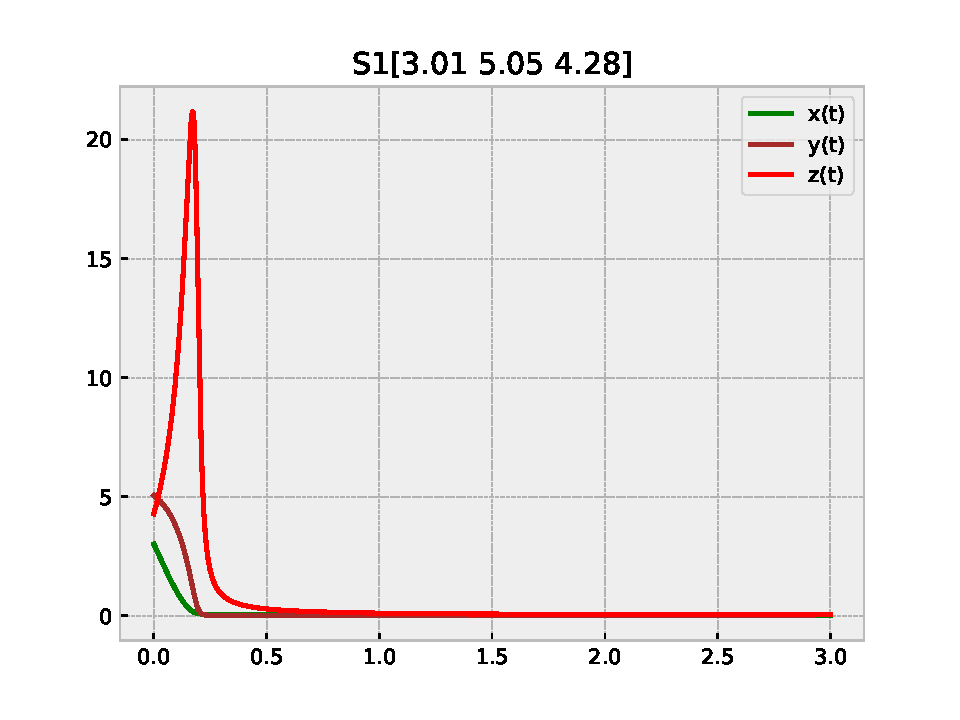
\includegraphics[width=\textwidth]{Simulations/S1[3.01 5.05 4.28].pdf}
		\label{fig:grafica1}
	\end{subfigure}%
	\begin{subfigure}[b]{0.5\textwidth}
		\centering
		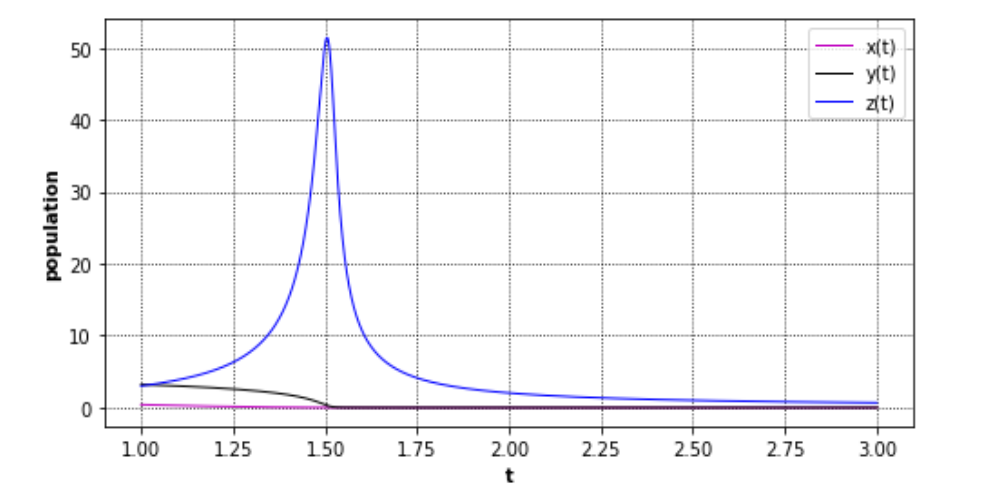
\includegraphics[width=\textwidth]{GraficasPaper/S1[1].png}
		\label{fig:grafica12}
	\end{subfigure}
	\caption{S1 con valores iniciales [3.01 5.05 4.28]}
	\label{fig:comparacion1}
\end{figure}

\begin{figure}[H]
	\centering
	\begin{subfigure}[b]{0.5\textwidth}
		\centering
		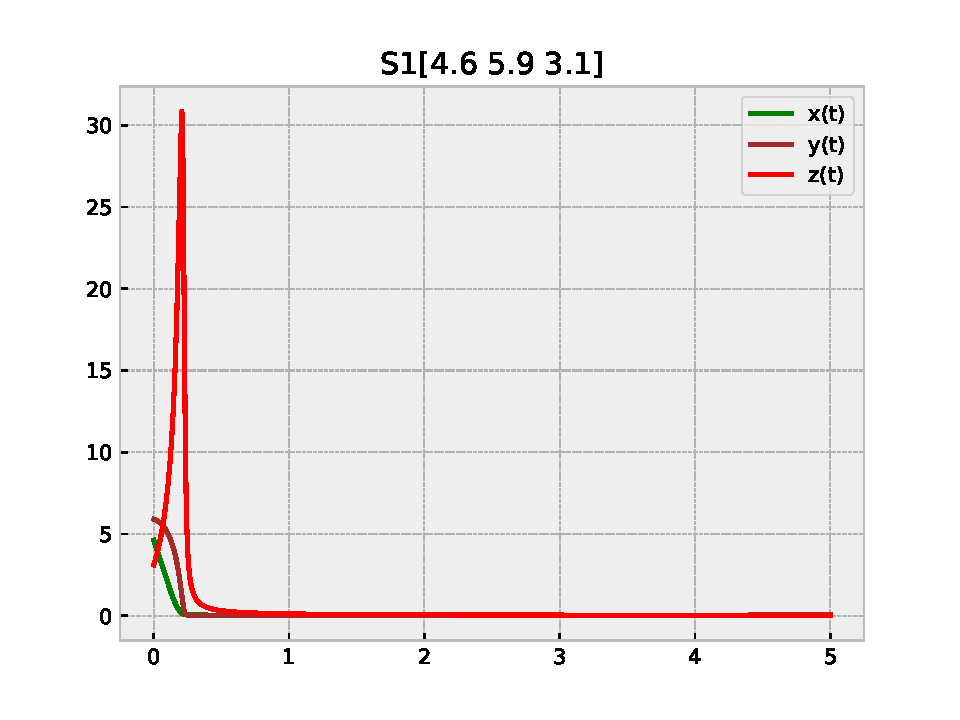
\includegraphics[width=\textwidth]{Simulations/S1[4.6 5.9 3.1].pdf}
	
		\label{fig:comparativa21}
	\end{subfigure}%
	\begin{subfigure}[b]{0.5\textwidth}
		\centering
		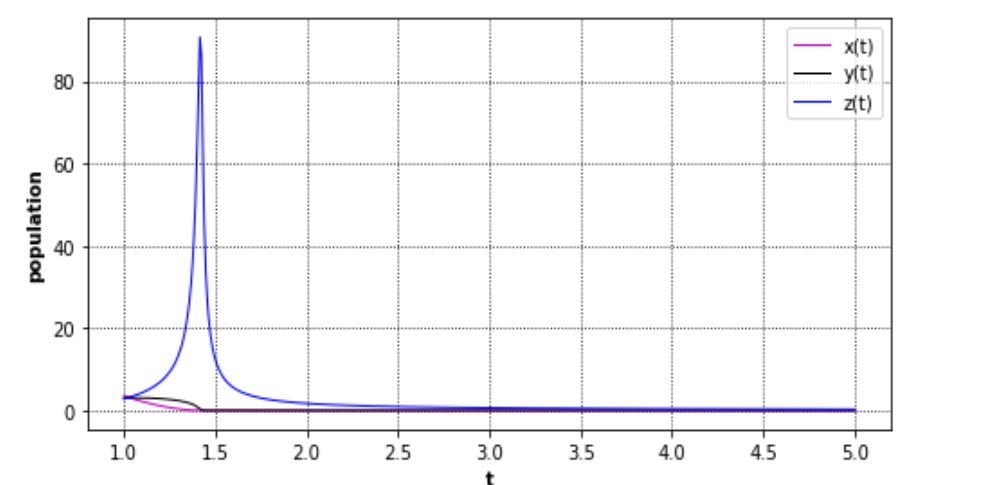
\includegraphics[width=\textwidth]{GraficasPaper/S1[2].png}
		\label{fig:comparativa22}
	\end{subfigure}
	\caption{S1 con valores iniciales [4.6 5.9 3.1]}

	\label{fig:comparacion2}
\end{figure}

\begin{figure}[h]
	\centering
	\begin{subfigure}[b]{0.5\textwidth}
		\centering
		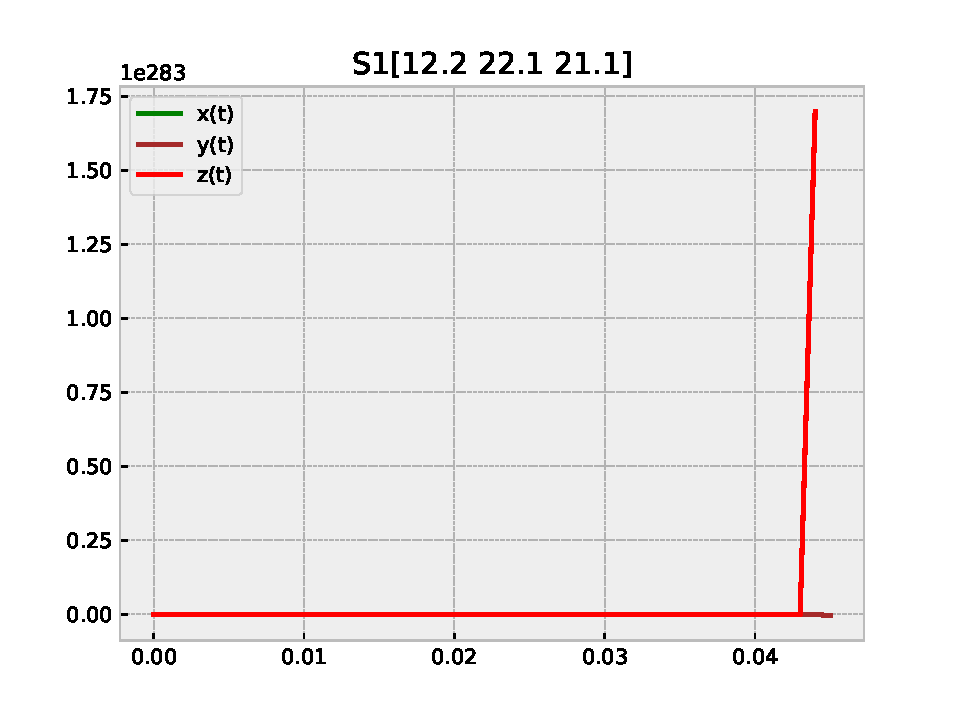
\includegraphics[width=\textwidth]{Simulations/S1[12.2 22.1 21.1].pdf}
	
		\label{fig:comparativa31}
	\end{subfigure}%
	\begin{subfigure}[b]{0.5\textwidth}
		\centering
		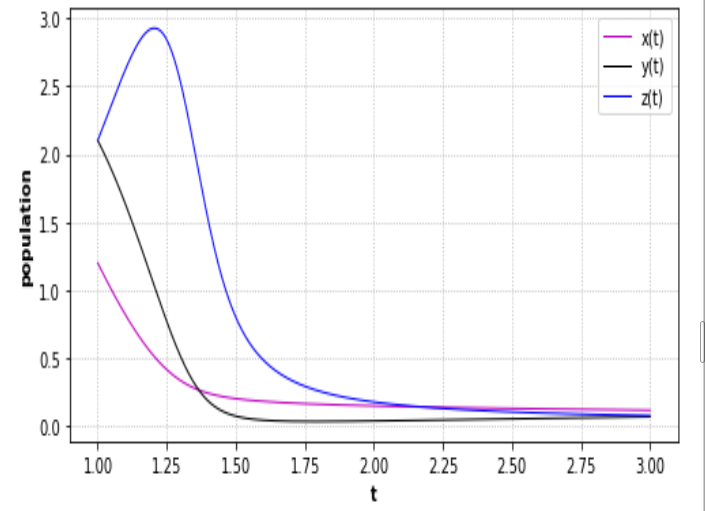
\includegraphics[width=\textwidth]{GraficasPaper/S1[3].png}
		\label{fig:comparativa32}
	\end{subfigure}
	\caption{S1 con valores iniciales [12.2 22.1 21.1], se experimentaron problemas de overflow.}

	\label{fig:comparacion3}
\end{figure}

\begin{figure}[h]
	\centering
	\begin{subfigure}[b]{0.5\textwidth}
		\centering
		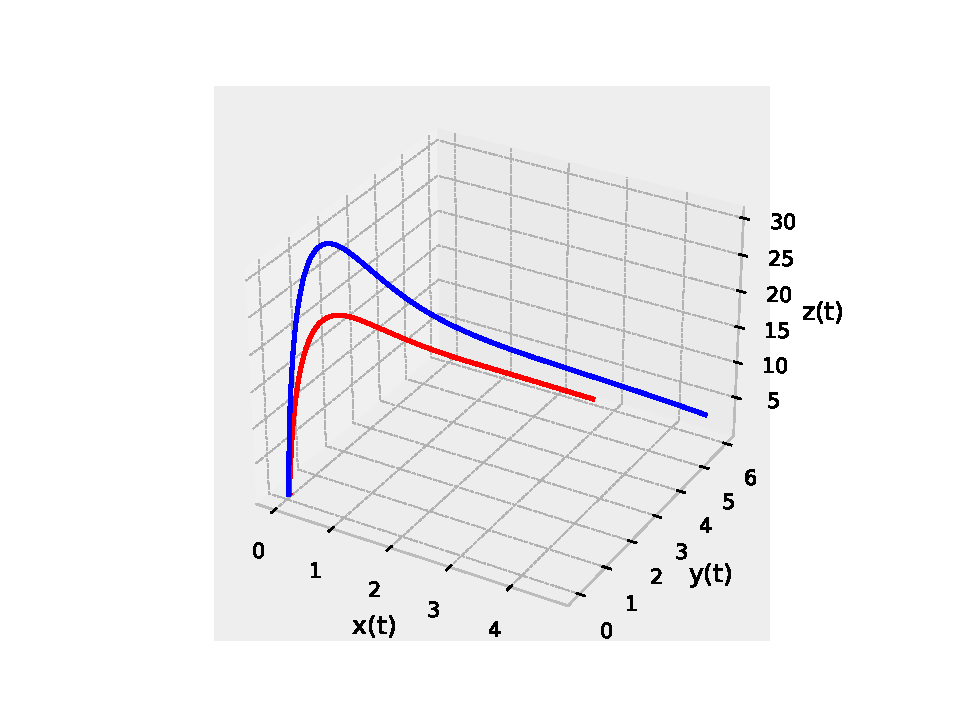
\includegraphics[width=\textwidth]{Simulations/S13d.pdf}
	
		\label{fig:comparativa3D1}
	\end{subfigure}%
	\begin{subfigure}[b]{0.5\textwidth}
		\centering
		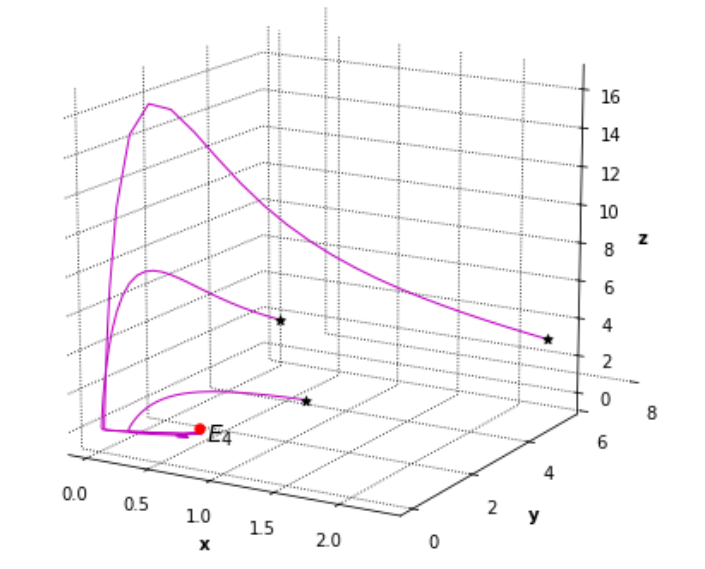
\includegraphics[width=\textwidth]{GraficasPaper/S1[3d].png}
		\label{fig:comparativa3D12}
	\end{subfigure}
	\caption{S1 3D, se experimentaron problemas de overflow.}

	\label{fig:comparacion4}
\end{figure}

\begin{figure}[htpb]
	\centering
	\begin{subfigure}[b]{0.5\textwidth}
		\centering
		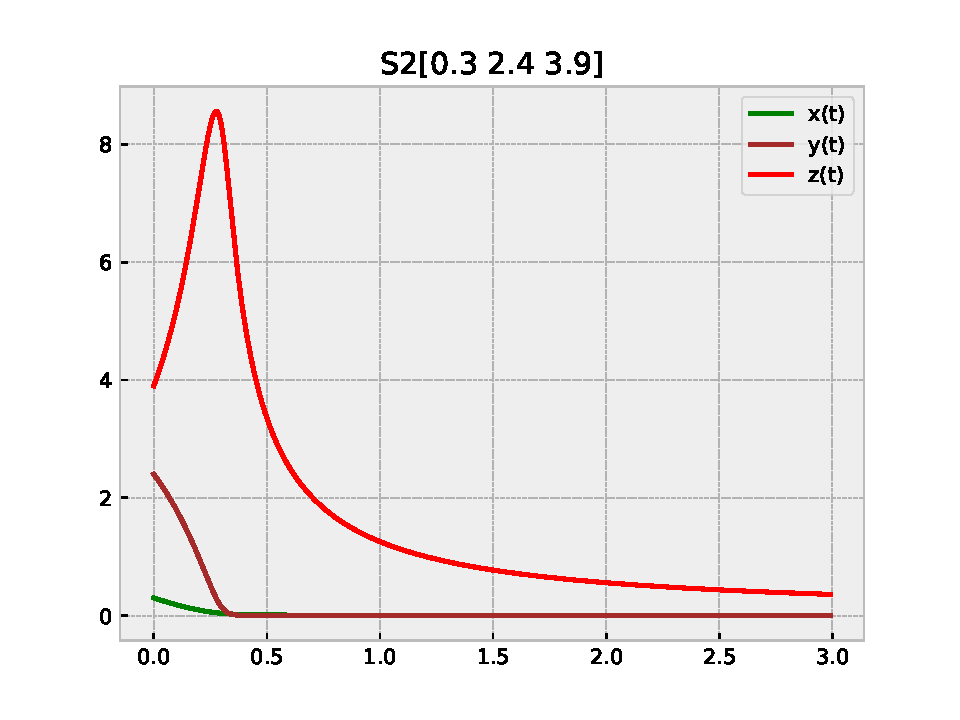
\includegraphics[width=\textwidth]{Simulations/S2[0.3 2.4 3.9].pdf}
	
		\label{fig:comparativa41}
	\end{subfigure}%
	\begin{subfigure}[b]{0.5\textwidth}
		\centering
		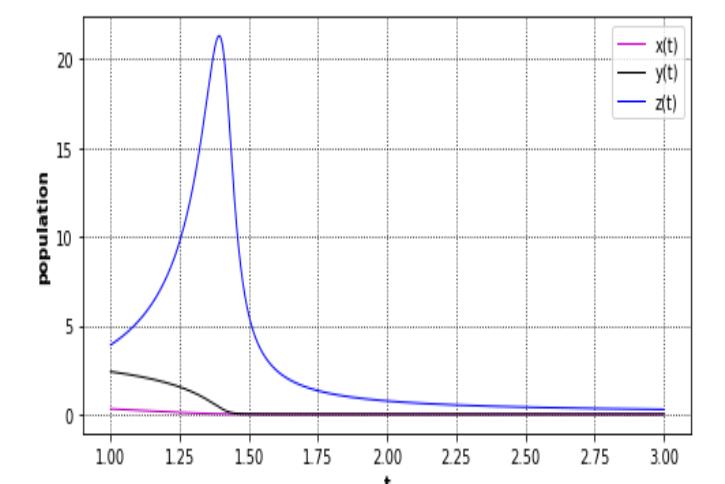
\includegraphics[width=\textwidth]{GraficasPaper/S2[1].png}
		\label{fig:comparativa42}
	\end{subfigure}
	\caption{S2 con valores iniciales [0.3 2.4 3.9]}

	\label{fig:comparacion5}
\end{figure}

\begin{figure}[h]
	\centering
	\begin{subfigure}[b]{0.5\textwidth}
		\centering
		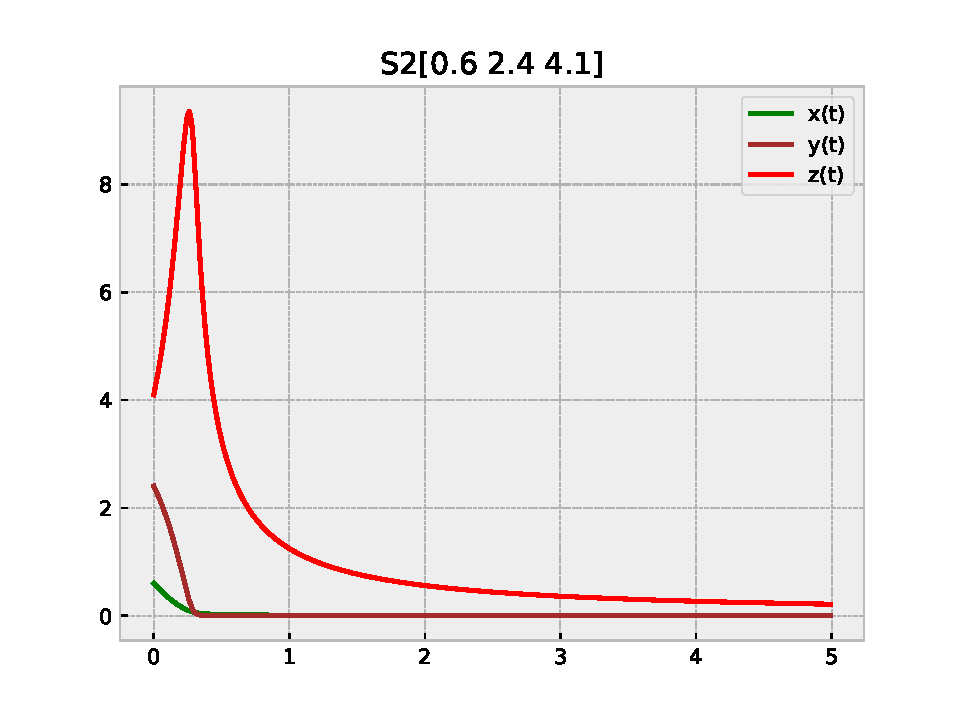
\includegraphics[width=\textwidth]{Simulations/S2[0.6 2.4 4.1].pdf}
	
		\label{fig:comparativa51}
	\end{subfigure}%
	\begin{subfigure}[b]{0.5\textwidth}
		\centering
		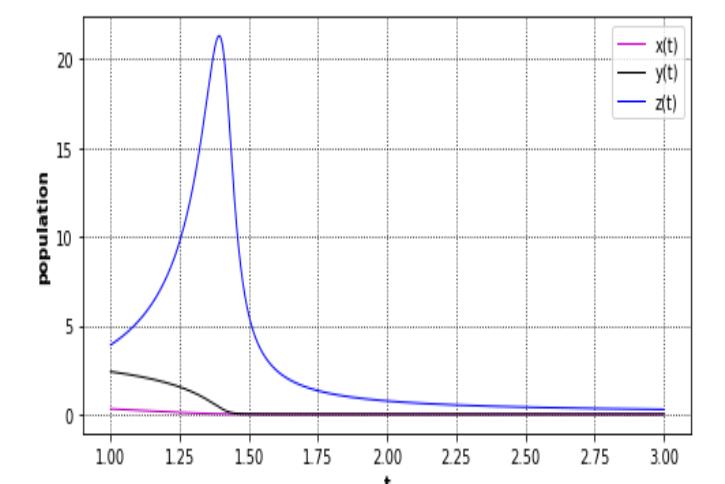
\includegraphics[width=\textwidth]{GraficasPaper/S2[1].png}
		\label{fig:comparativa52}
	\end{subfigure}
	\caption{S2 con valores iniciales [0.6 2.4 4.1]}

	\label{fig:comparacion6}
\end{figure}

\begin{figure}[h]
	\centering
	\begin{subfigure}[b]{0.5\textwidth}
		\centering
		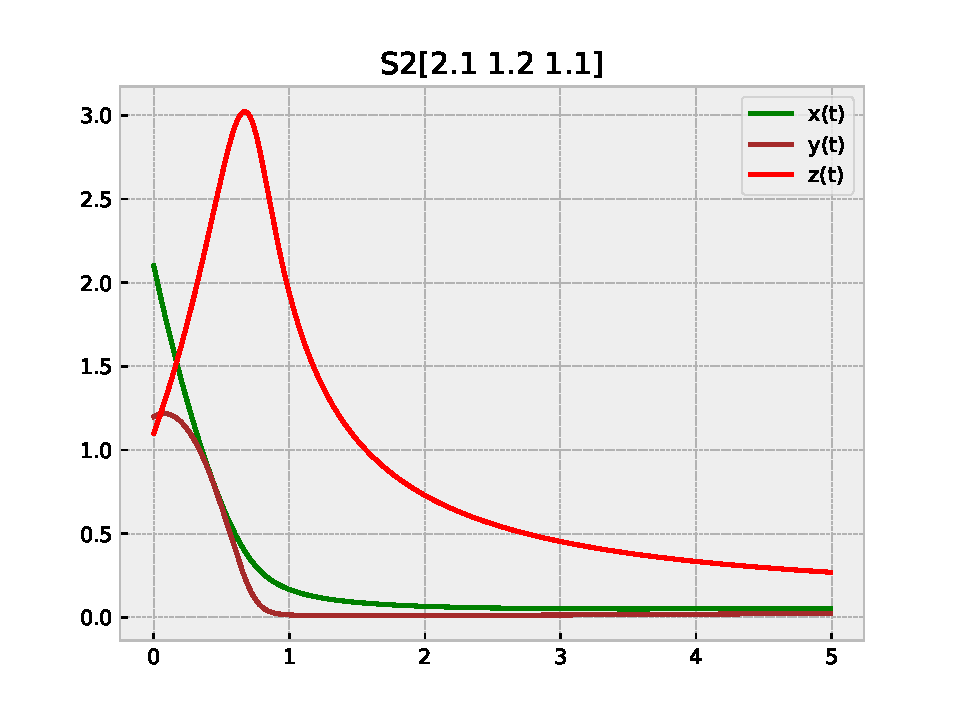
\includegraphics[width=\textwidth]{Simulations/S2[2.1 1.2 1.1].pdf}
	
		\label{fig:comparativa61}
	\end{subfigure}%
	\begin{subfigure}[b]{0.5\textwidth}
		\centering
		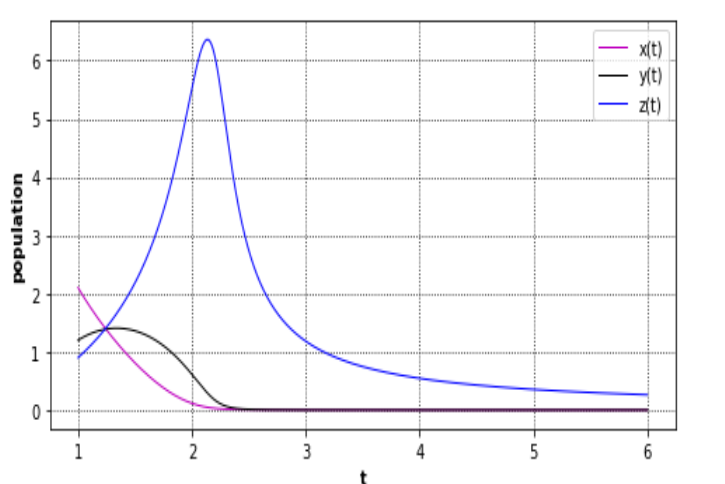
\includegraphics[width=\textwidth]{GraficasPaper/S2[3].png}
		\label{fig:comparativa62}
	\end{subfigure}
	\caption{S2 con valores iniciales [2.1 1.2 1.1]}

	\label{fig:comparacion7}
\end{figure}

\begin{figure}[h]
	\centering
	\begin{subfigure}[b]{0.5\textwidth}
		\centering
		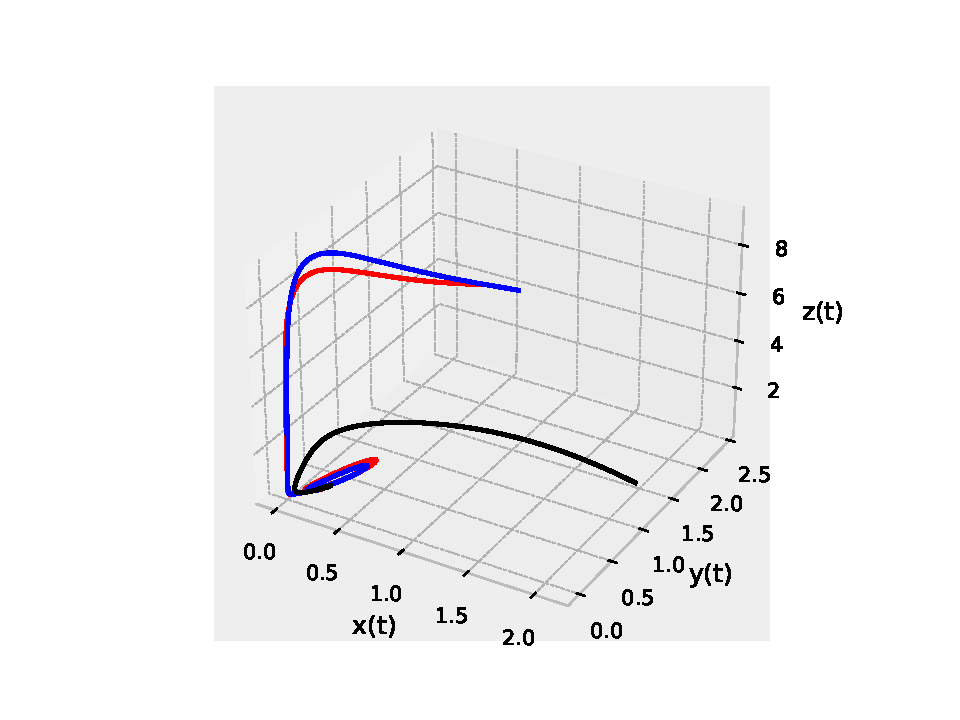
\includegraphics[width=\textwidth]{Simulations/S23d.pdf}
	
		\label{fig:comparativa3D2}
	\end{subfigure}%
	\begin{subfigure}[b]{0.5\textwidth}
		\centering
		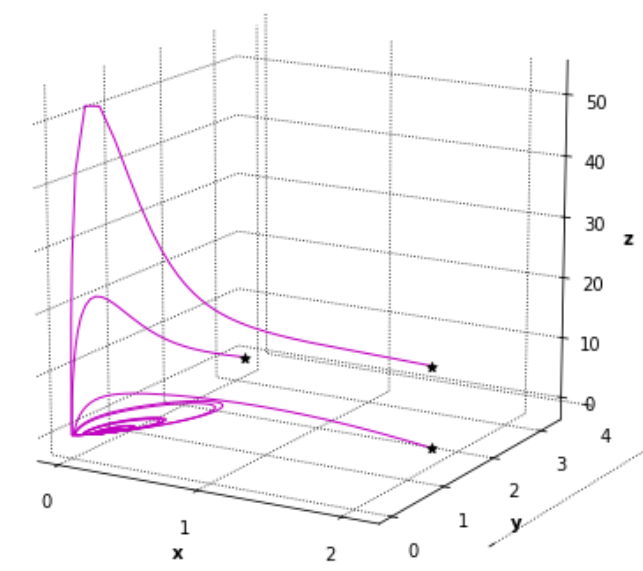
\includegraphics[width=\textwidth]{GraficasPaper/S2[3d3].png}
		\label{fig:comparativa3D22}
	\end{subfigure}
	\caption{S2 con valores iniciales}

	\label{fig:comparacion8}
\end{figure}

\begin{figure}[h]
	\centering
	\begin{subfigure}[b]{0.5\textwidth}
		\centering
		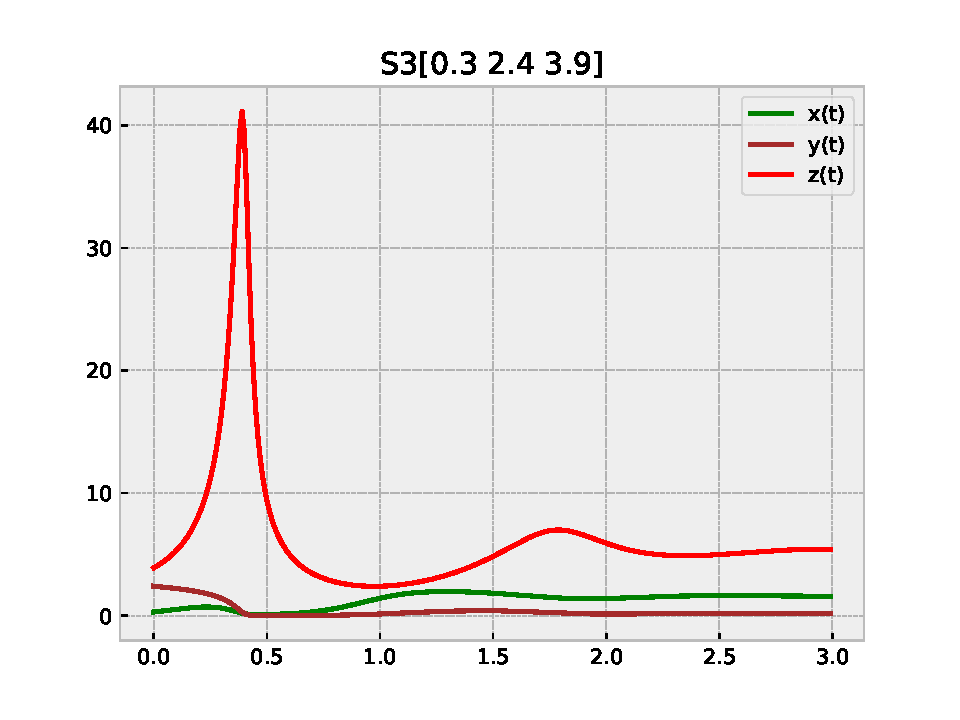
\includegraphics[width=\textwidth]{Simulations/S3[0.3 2.4 3.9].pdf}
	
		\label{fig:comparativa71}
	\end{subfigure}%
	\begin{subfigure}[b]{0.5\textwidth}
		\centering
		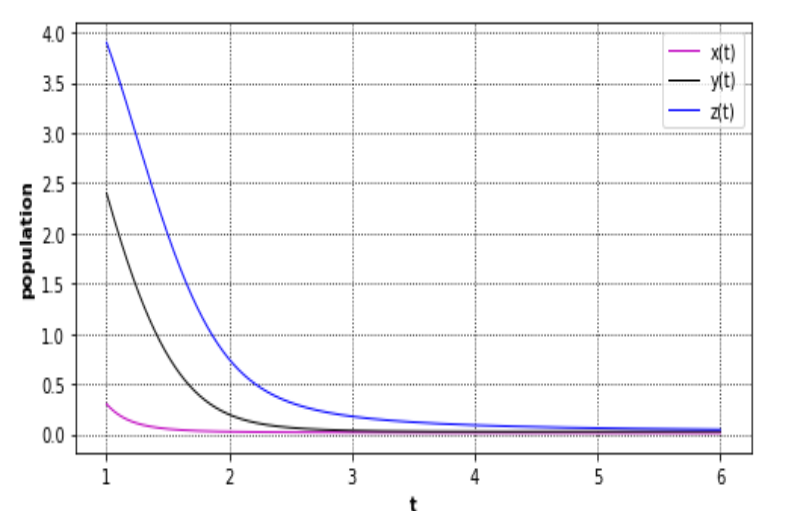
\includegraphics[width=\textwidth]{GraficasPaper/S3[1].png}
		\label{fig:comparativa72}
	\end{subfigure}
	\caption{S3 con valores iniciales [0.3 2.4 3.9]}

	\label{fig:comparacion9}
\end{figure}

\begin{figure}[h]
	\centering
	\begin{subfigure}[b]{0.5\textwidth}
		\centering
		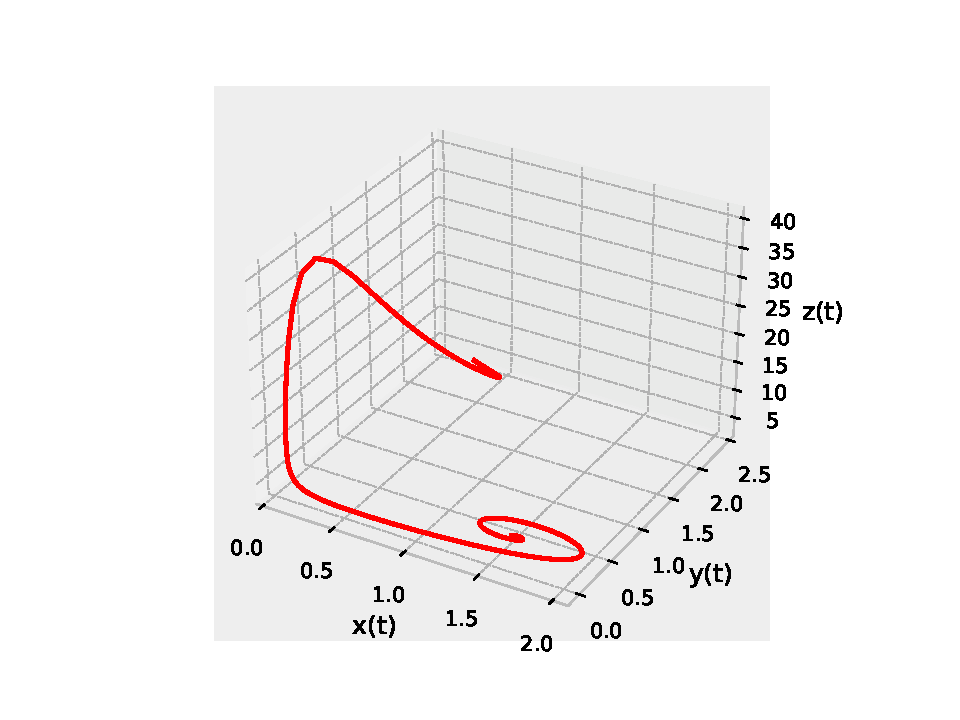
\includegraphics[width=\textwidth]{Simulations/S33d.pdf}
	
		\label{fig:comparativa3D31}
	\end{subfigure}%
	\begin{subfigure}[b]{0.5\textwidth}
		\centering
		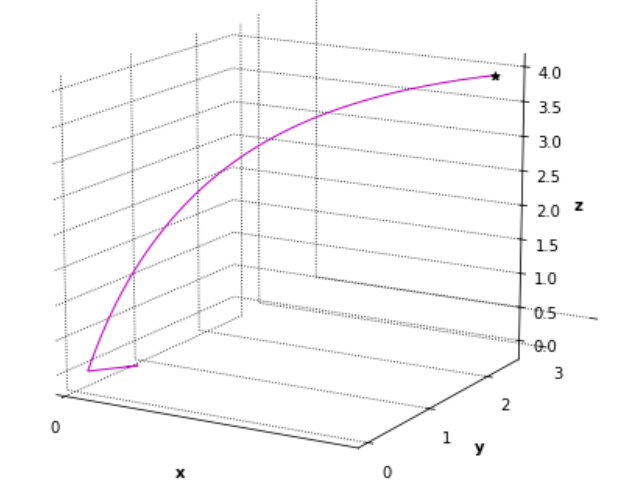
\includegraphics[width=\textwidth]{GraficasPaper/S3[3d].png}
		\label{fig:comparativa3D32}
	\end{subfigure}
	\caption{S3 3D}

	\label{fig:comparacion10}
\end{figure}

\begin{figure}[h]
	\centering
	\begin{subfigure}[b]{0.5\textwidth}
		\centering
		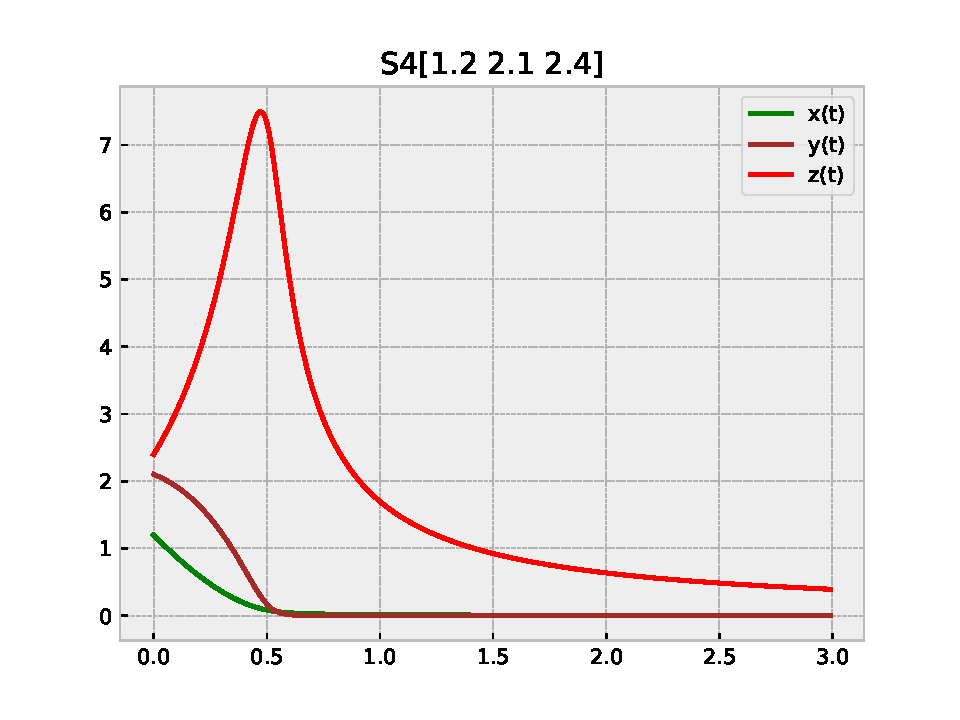
\includegraphics[width=\textwidth]{Simulations/S4[1.2 2.1 2.4].pdf}
	
		\label{fig:comparativa81}
	\end{subfigure}%
	\begin{subfigure}[b]{0.5\textwidth}
		\centering
		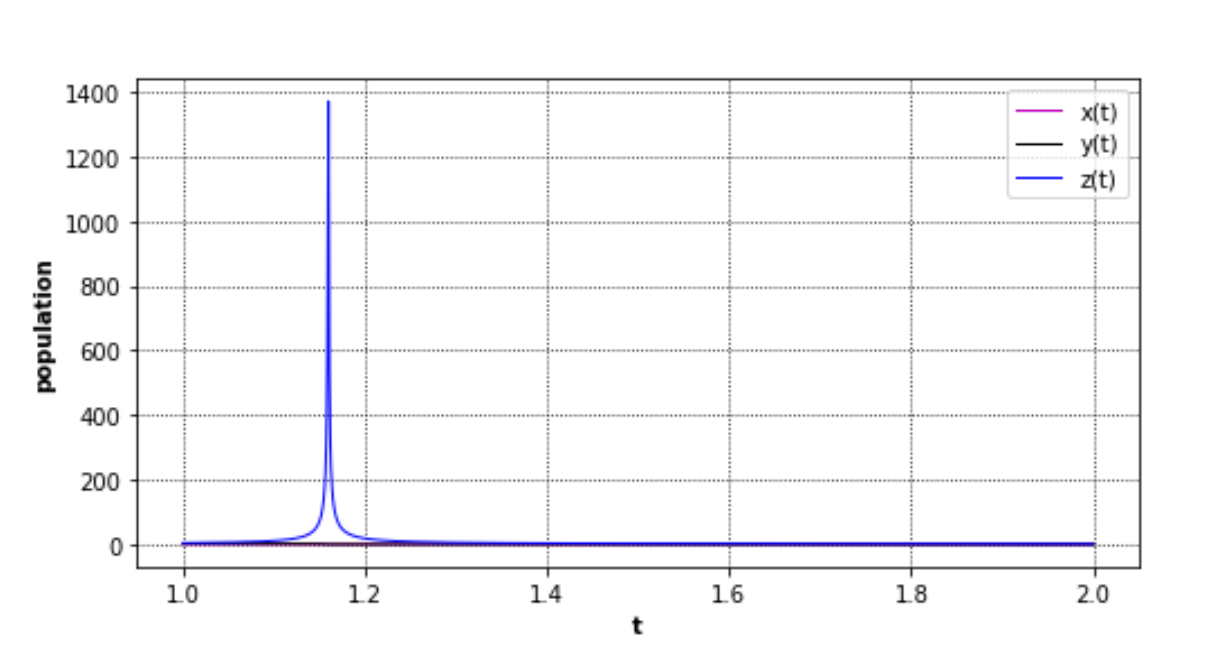
\includegraphics[width=\textwidth]{GraficasPaper/S4[1].png}
		\label{fig:comparativa82}
	\end{subfigure}
	\caption{S4 con valores iniciales [1.2 2.1 2.4]}

	\label{fig:comparacion11}
\end{figure}

\begin{figure}[h]
	\centering
	\begin{subfigure}[b]{0.5\textwidth}
		\centering
		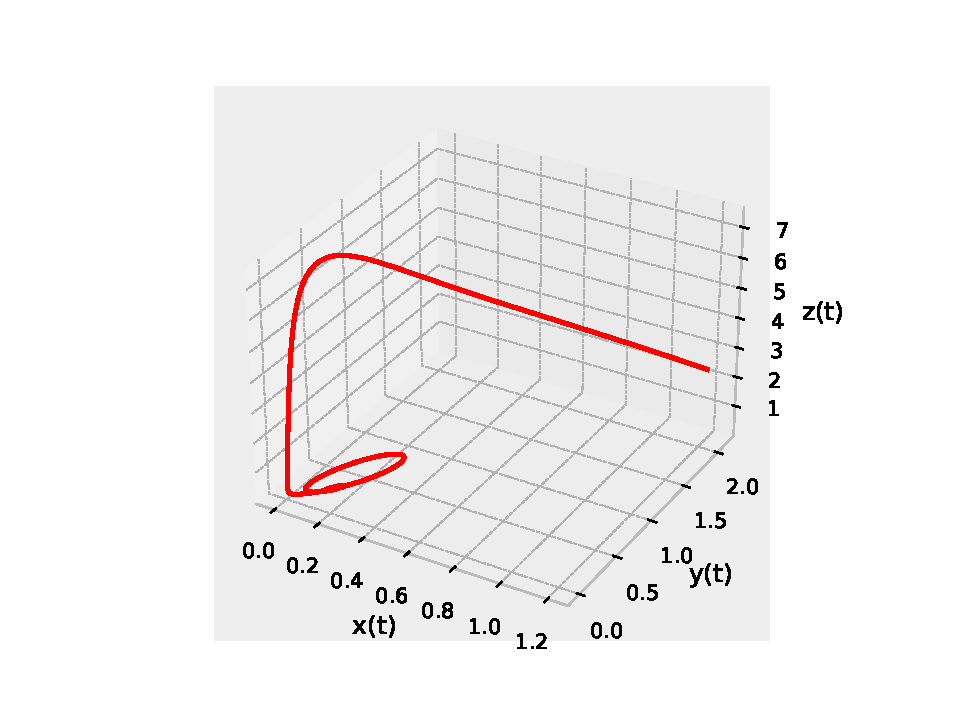
\includegraphics[width=\textwidth]{Simulations/S43d.pdf}
	
		\label{fig:comparativa3D41}
	\end{subfigure}%
	\begin{subfigure}[b]{0.5\textwidth}
		\centering
		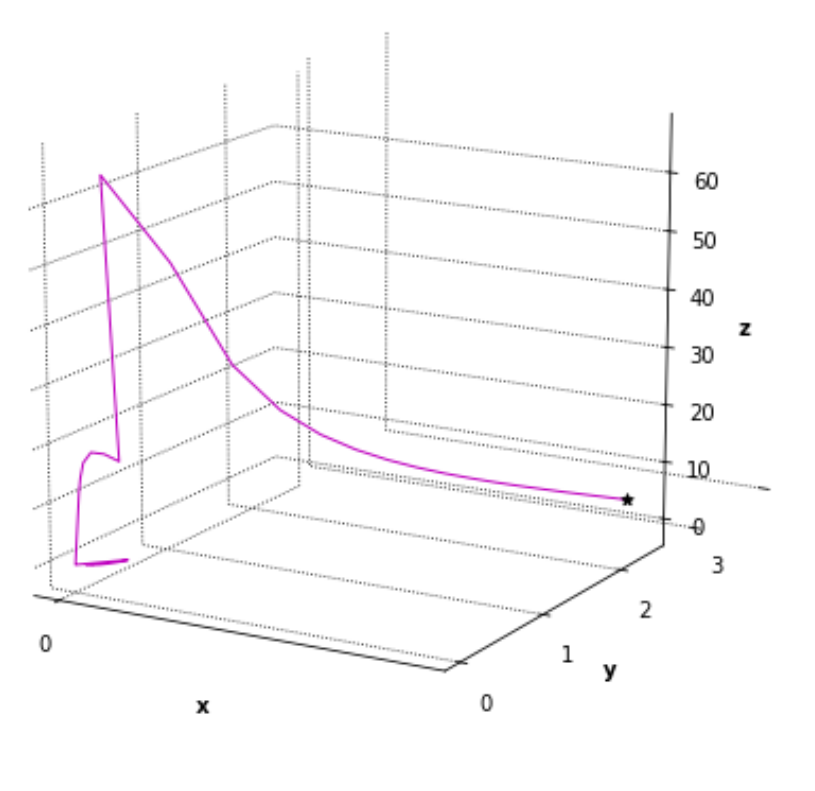
\includegraphics[width=\textwidth]{GraficasPaper/S4[3d].png}
		\label{fig:comparativa3D42}
	\end{subfigure}
	\caption{S4 3D}

	\label{fig:comparacion12}
\end{figure}

\begin{figure}[h]
	\centering
	\begin{subfigure}[b]{0.5\textwidth}
		\centering
		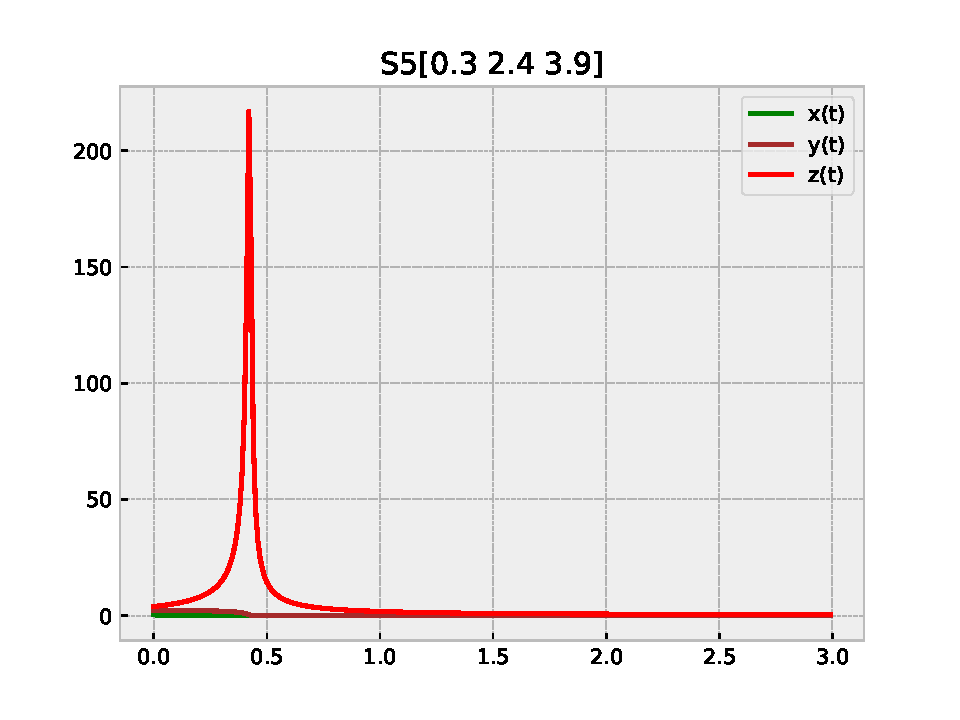
\includegraphics[width=\textwidth]{Simulations/S5[0.3 2.4 3.9].pdf}
	
		\label{fig:comparativa91}
	\end{subfigure}%
	\begin{subfigure}[b]{0.5\textwidth}
		\centering
		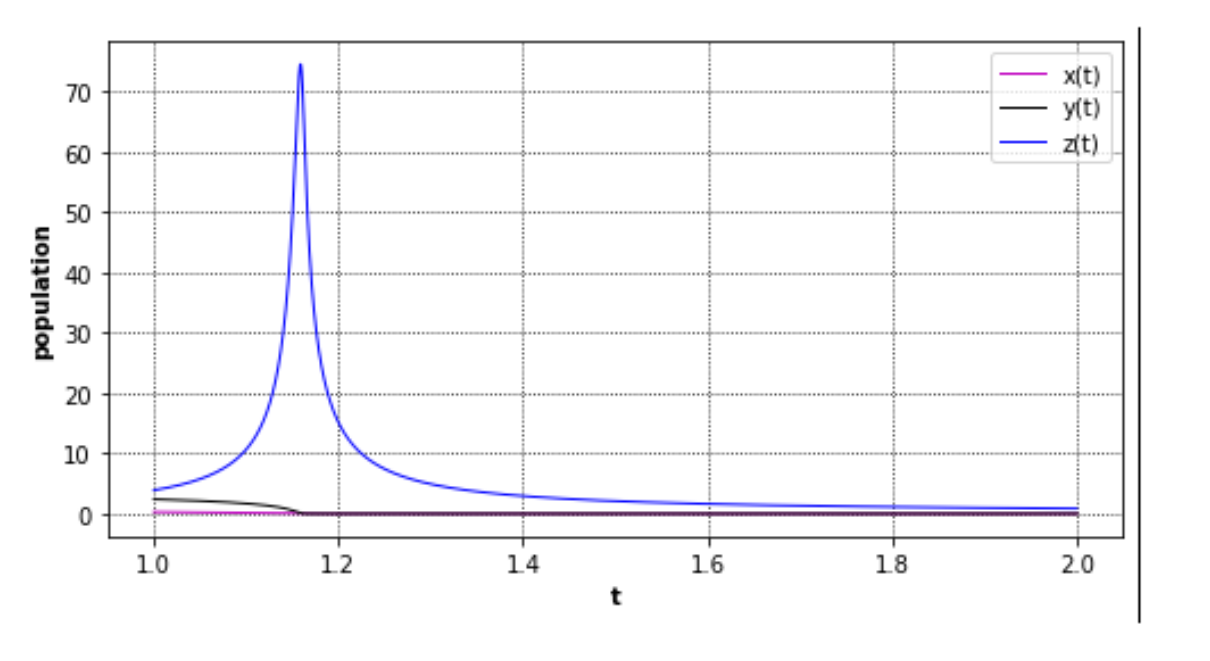
\includegraphics[width=\textwidth]{GraficasPaper/S5[1].png}
		\label{fig:comparativa92}
	\end{subfigure}
	\caption{S5 con valores iniciales [0.3 2.4 3.9]}

	\label{fig:comparacion13}
\end{figure}




\FloatBarrier
\subsection{M\'etodos y algoritmos utilizados}
Códigos del método de Euler y de Runge-Kutta utilizados para la solución del sistema:
\begin{verbatim}
	def euler(f, c, h, time):
    x = [c]
    t = [0]
    n = int(time//h)

    for i in range(n):
        x.append(x[i] + h*f(t, x[i]))
        t.append(t[i]+h)
    
    x = np.array(x)
    return t, x


	
	def runge_kutta(f, c, h, time):
    x = [c]
    t = [0]
    n = int(time//h)
    
    for i in range(n):
        k1 = f(t[i], x[i])
        k2 = f(t[i] + h/2, x[i] + 0.5*h*k1)
        k3 = f(t[i] + h/2, x[i] + 0.5*h*k2)
        k4 = f(t[i] + h, x[i] + h*k3)
        t.append(t[i] + h)
        x.append(x[i] + h/6*(k1 + 2*k2 + 2*k3 + k4))

    x = np.array(x)
    return t, x
	
	
	# Parametros del sistema (positivos)
	r = 0.82
	alpha = 1.56
	beta = 0.87
	rho = 1.38
	m = 0.13
	mu = 0.11
	eta = 2.41
	alpha1 = 1.12
	eta1 = 1.83
	k = 12
	
	
	def f1(x, y, z):
		return x*(r*(k-x)/k-beta-alpha*z)
	
	
	def f2(x, y, z):
		return beta*x-y*((eta*z)/(y+m)-mu)
	
	
	def f3(x, y, z):
		return z*(alpha1*x+rho*z-(eta1*y)/(y+m))
	
\end{verbatim}

\section*{Conclusiones}
Este estudio proporciona una comprensi\'on más profunda de las complejas interacciones entre los depredadores y sus presas en
los ecosistemas naturales. Los resultados obtenidos pueden ser \'utiles para predecir y manejar las poblaciones de presas y
depredadores en diferentes entornos y para comprender mejor los efectos del cambio clim\'atico y otros factores ambientales
en estas interacciones. \par
Durante este trabajo hemos aprendido sobre varios temas relacionados con las ecuaciones diferenciales
y el modelado matemático. Hemos aprendido a resolver sistemas de ecuaciones diferenciales utilizando diferentes
métodos numéricos, como el método de Euler o el método de Runge-Kutta. Además, hemos aprendido a modelar la interacción entre
dos especies, analizando la dinámica de este modelo y estudiando su estabilidad. También hemos aprendido a utilizar las matemáticas
para modelar problemas del mundo real y la importancia de los modelos matemáticos en varias disciplinas. Hemos utilizado diferentes
programas de simulación numérica, como Python, para resolver ecuaciones diferenciales y visualizar los resultados, lo que
nos ha ayudado a entender mejor los modelos matemáticos y hacer predicciones sobre el comportamiento de los sistemas. Hemos estudiado
la estabilidad de sistemas dinámicos, utilizando técnicas como el análisis de estabilidad lineal y el método de Routh-Hurwitz, y hemos
desarrollado habilidades investigativas, como la capacidad de buscar y analizar información relevante, trabajar en equipo, elaborar y
presentar informes técnicos, y utilizar herramientas matemáticas y de programación para resolver problemas. \par
Creemos que es importante seguir explorando los modelos matemáticos y las técnicas de simulación numérica para entender mejor
los sistemas dinámicos y predecir su comportamiento en diferentes áreas, como la biología, la física, la ingeniería y
la economía. Este trabajo nos ha dado una buena base para continuar explorando estos temas en el futuro y desarrollar
nuevas investigaciones en este campo.


\defbibheading{Referencias}{\section*{Referencias}}
\defbibheading{Bibliografía}{\section*{Bibliografía}}

\printbibliography[heading=Referencias, type=article]
\renewcommand{\theenumiv}{}
\DeclareFieldFormat{labelnumberwidth}{}
\printbibliography[heading=Bibliografía, type=book, resetnumbers=true]
\nocite{edwards_differential_2008}
\nocite{upadhyay_introduction_2013}



\section*{Agradeciemientos}
Agradecemos al claustro de profesores de la asignatura por su esfuerzo y tiempo empleado en nosotros.

\appendix

\section{Anexos} \label{app:Anexos}

\begin{center}
	Modelo propuesto por Huenchucona, Falconi y Vidal
	\\
\end{center}

\begin{equation} \label{twoPreyonePredator_Falconi}
	\begin{gathered}
		\frac{d x_1}{d t}=r x_1\left(1-\frac{x_1}{K}\right)-\beta x_1-\frac{\beta_1 x_1 y}{1+m_1 x_1^2+n_1 x_2} \\
		\frac{d x_2}{d t}=\beta x_1-\frac{\beta_2 x_2 y}{1+m_2 x_1+n_2 x_2}-\mu_1 x_2                           \\
		\frac{d y}{d t}=\frac{\alpha_1 \beta_1 x_1 y}{1+m_1 x_1^2+n_1 x_2}+\frac{\alpha_2 \beta_2 x_2 y}{1+m_2 x_1+n_2 x_2}-\mu_2 y
	\end{gathered}
\end{equation}
\\
\begin{center}
	Modelo propuesto por Savitri y Abadi
	\\
\end{center}
\begin{equation} \label{Holling1y2_Abadi}
	\begin{gathered}
		\frac{d x_1}{d t}=r x_1\left(1-\frac{x_1}{K}\right)-\beta x_1-\alpha x_1 y \\
		\frac{d x_2}{d t}=\beta x_1-\frac{\varepsilon x_2 y}{1+m x_2}-\mu_1 x_2 \\
		\frac{d y}{d t}=\frac{\gamma \varepsilon x_2 y}{1+m x_2}-\mu_2 y
	\end{gathered}
\end{equation}

\begin{center}
	Modelo propuesto por Castellanos y Chan-López
\end{center}
\begin{equation} \label{Holling1y2_Castellanos}
	\begin{gathered}
		\frac{d x}{d t}=\rho x\left(1-\frac{x}{k}\right)-a_1 x \\
		\frac{d y}{d t}=c a_1 x y-d y-\frac{a_2 y z}{y+b_2} \\
		\frac{d z}{d t}=\alpha z^2-\frac{\beta z^2}{y+b_2}
	\end{gathered}
\end{equation}

\begin{center} 
	Script en Python para calcular la Jacobiana y Routh-Hurwitz.
\end{center}
\begin{verbatim}
	# Define the variables
	x, y, z, r, k, b, a, n, m, u, a1, p, n1 = symbols('x y z r k b a n m u a1 p n1')
	
	# Define the equations
	eq1 = r*x*(1-x/k) - b*x - a*x*z
	eq2 = b*x - (n*y*z)/(y+m) - u*y
	eq3 = a1*x*z + p*z**2 - (n1*z**2)/(y+m)
	
	# Verify if E2 is an equilibrium point
	dx = sp.simplify(sp.Subs(eq1, (x,y,z), (((k*(r-b))/r),
					 (b*k*(r-b))/(u*r), 0)).doit())
	dy = sp.simplify(sp.Subs(eq2, (x,y,z), (((k*(r-b))/r),
					 (b*k*(r-b))/(u*r), 0)).doit())
	dz = sp.simplify(sp.Subs(eq3, (x,y,z), (((k*(r-b))/r),
					 (b*k*(r-b))/(u*r), 0)).doit())
	print("E2 is an equilibrium point:", {dx==0 and dy==0 and dz==0})
	
	separator = '- - '*25
	print(separator)
	
	# Define the variables as a list
	variables = [x, y, z]
	
	# Define the equations as a list
	equations = [eq1, eq2, eq3]
	
	# Create the Jacobian matrix
	Jacobian = Matrix(equations).jacobian(variables)
	Jacobian = sp.simplify(Jacobian)
	print("Jacobian matrix:")
	print(Jacobian)
	
	print(separator)
	
	# Verify the local stability of the equilibrium point E1
	E1=sp.Subs(Jacobian, (x,y,z), (0,0,0)).doit()
	E1=sp.simplify(E1)
	eigenvaluesE1 = list(sp.Matrix.eigenvals(E1, simplify=True, multiple=True))
	print(f"Jacobian(E1): {E1}")
	print(f"Eigenvalues of Jacobian(E1): {eigenvaluesE1}")
	
	print(separator)
	
	# Verify the local stability of the equilibrium point E2
	E2=sp.Subs(Jacobian, (x,y,z), (((k*(r-b))/r), (b*k*(r-b))/(u*r), 0)).doit()
	E2=sp.simplify(E2)
	eigenvaluesE2 = list(sp.Matrix.eigenvals(E2).keys())
	print(f"Jacobian(E2): {E2}")
	print(f"Eigenvalues of Jacobian(E2): {eigenvaluesE2}")
	
	print(separator)
	
	
	# Checking the Routh–Hurwitz criterion for the E3 stability
	A1=sp.simplify(-Jacobian[0,0]-Jacobian[1,1]-Jacobian[2,2])
	print(f"A1: {A1}")
	
	print(separator)
	
	A2=sp.simplify(-Jacobian[0,1]*Jacobian[1,0]-Jacobian[0,2]*Jacobian[2,0]
					-Jacobian[1,2]*Jacobian[2,1] +Jacobian[1,1]*Jacobian[2,2]
					+Jacobian[0,0]*(Jacobian[1,1]+Jacobian[2,2]))
	print(f"A2: {A2}")
	
	print(separator)
	
	A3=sp.simplify(Jacobian[0,2]*(Jacobian[1,1]*Jacobian[2,0]-Jacobian[1,0]
								*Jacobian[2,1])+Jacobian[0,1]*(Jacobian[1,0]*Jacobian[2,2]
								-Jacobian[1,2]*Jacobian[2,0])+Jacobian[0,0]*(Jacobian[1,2]*Jacobian[2,1]
								-Jacobian[1,1]*Jacobian[2,2]))
	print(f"A3: {A3}")
	
	print(separator)
	
	Hurwitz = Matrix([[0,0,0],[0,0,0],[0,0,0]])
	Hurwitz[0,0]=A1
	Hurwitz[0,1]=A3
	Hurwitz[1,0]=1
	Hurwitz[1,1]=A2
	Hurwitz[2,1]=A1
	Hurwitz[2,2]=A3
	
	H1=A1
	# H1Subs=sp.Subs(H1, (r, k, b, a, n, m ,u, a1, p, n1), 
					(0.82,12,0.87, 1.56, 2.41, 0.13, 0.11, 1.12, 1.38, 1.83)).doit()
	print(f"H1: {H1}")
	
	print(separator)
	
	H2=A1*A2-A3
	# H2Subs=sp.Subs(H2, (r, k, b, a, n, m ,u, a1, p, n1), 
					(0.82,12,0.87, 1.56, 2.41, 0.13, 0.11, 1.12, 1.38, 1.83)).doit()
	print(f"H2: {H2}")
	
	print(separator)
	
	H3=A1*A2*A3-A3*A3
	# H3Subs=sp.Subs(H3, (r, k, b, a, n, m ,u, a1, p, n1), 
					(0.82,12,0.87, 1.56, 2.41, 0.13, 0.11,
					 1.12, 1.38, 1.83)).doit()
	print(f"H3: {H3}")
\end{verbatim}
\label{Jacobian}

\end{document}

